%% This is an example first chapter.  You should put chapter/appendix that you
%% write into a separate file, and add a line \include{yourfilename} to
%% main.tex, where `yourfilename.tex' is the name of the chapter/appendix file.
%% You can process specific files by typing their names in at the 
%% \files=
%% prompt when you run the file main.tex through LaTeX.

\singlespacing{

\chapter{Design Hierarchy}

\section{Elements}

At the lowest level, bulk materials in the form of \textit{elements} are assembled together to form multimaterial assemblies.  
Elemental components are on the order of ~1um\textsuperscript{3}.

\section{Functions}

Assemblies of \textit{elements} form components called \textit{functions}.
Functional Components are on the order of ~1mm\textsuperscript{3}.

degrees of freedom (function) + interface

\section{Modules}

\section{Complexes}

\section{Design Hierarchy in Biology}

\begin{sidewaysfigure}
  \includegraphics[width=\textwidth,height=\textheight,keepaspectratio]{ProteinHierarchy.png}
  \caption{Hierarchical breakdown of protein complexes (complexes) into proteins (modules), amino acids (functions), and atoms (elements).}
  \label{fig:ProteinHierarchy}
\end{sidewaysfigure}


Currently, the only known example of a physical, self-replicating system is the biology that has evolved on Earth.  Though we observe some slight variation across species, all biological self replication involves the use of protein machinery (called \textit{protein complexes}) built primarily from a small set of amino acid building blocks.\\

The construction of protein complexes takes place in a hierarchical fashion.  Figure \ref{fig:ProteinHierarchy} describes the hierarchical breakdown of protein complexes in terms of the four levels of hierarchy established earlier in this chapter; protein complexes (complex-level objects) are decomposed into proteins (modules), then into amino acids (functions), and finally into atomic elements (elements).  This hierarchical breakdown is slightly different from the primary/secondary/tertiary/quaternary structures typically used to discuss the levels of protein description.  The similarity of some of the biological nomenclature to our own hierarchical nomenclature is due to the fact that it was derived from the biological model.

\subsection{Elements, Functional Groups, and Functions}

At the most fundamental level, biological structures are composed of atoms of various elemental types.  Most biological molecules on Earth, especially those involved in protein synthesis and activation, are made from combinations of carbon, hydrogen, nitrogen, oxygen, phosphorus, and sulfur (CHNOPS).\\

Each element's unique position on the periodic table dictates its physical parameters, which have implications in higher-level structures formed from the elements.  These parameters include the element's mass, the number of covalent bonds it can form, the amount of unpaired electrons it contains in its outermost electron shell, the polarization of the bonds and molecules it forms with other elements, and the stability of its bonds in various environments.\\

Certain motifs of covalently bonded atoms form \textit{functional groups} within molecules.  Functional groups determine the ability of a molecule to undergo various characteristic reactions (addition, substitution, elimination, etc) in organic chemistry.  A subset of the important functional groups found in biochemistry are indicated in Figure \ref{fig:ProteinHierarchy}.  "R" indicates an arbitrary side-chain, where the functional group connects to the rest of the molecule.\\

\begin{figure}
  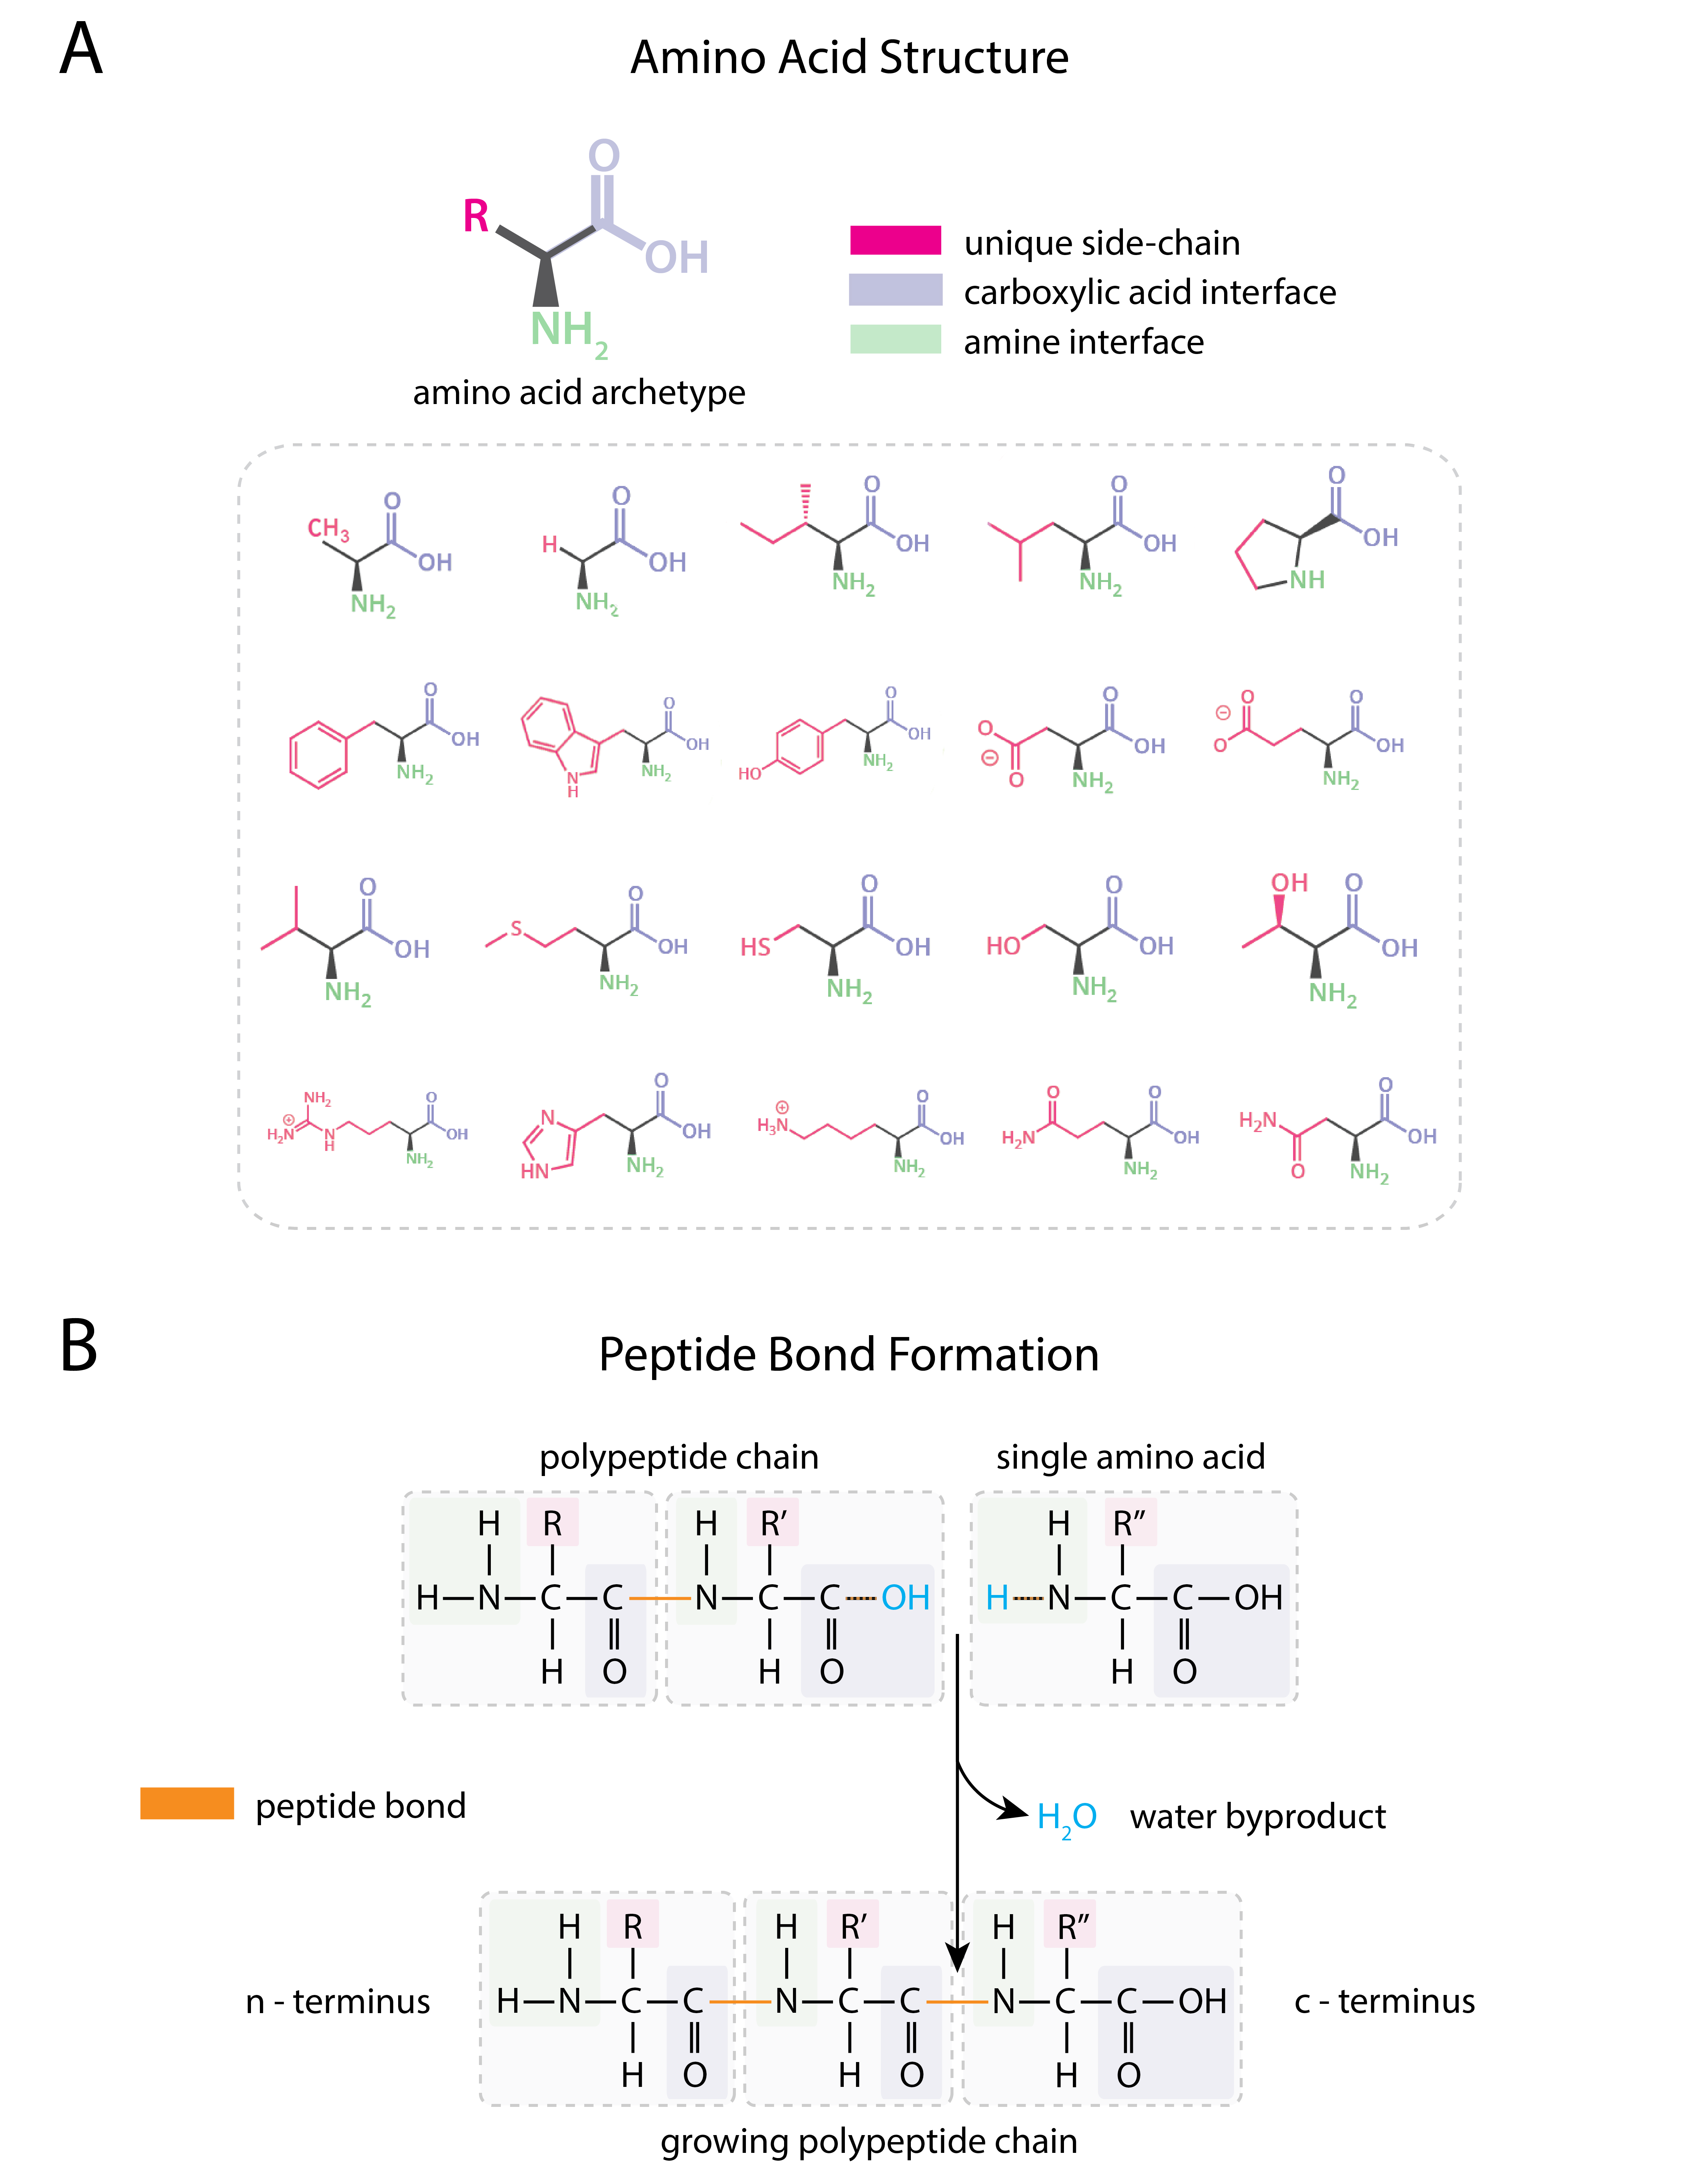
\includegraphics[width=\textwidth]{AminosInterface.png}
  \caption{(A) Decomposition of amino acids into carboxylic acid and amine interfaces and unique side-chain. (B) Formation of peptide bond at c-terminus (carboxylic acid group) of polypeptide chain with the n-terminus (amine group) of an amino acid. One molecule of water is produced as a byproduct of the peptide bonding reaction.  R, R', and R'' represent arbitrary amino acid side-chains.}
  \label{fig:AminosInterface}
\end{figure}

Amino acids are molecules that contain several functional groups.  As indicated in Figure \ref{fig:AminosInterface}A all amino acids contain a carboxylic acid (COOH) and an amine group (NH\textsubscript{2} or NRH).  The purpose of these groups is to form the peptide bonds between amino acids in a polypeptide chain.  Peptide bonding forms a covalent bond between two amino acids through a process called \textit{condensation}, with a single molecule of water created as a byproduct \ref{fig:AminosInterface}B.\\

The remaining portion of the amino acid (indicated by "R" in the amino acid archetype in Figure \ref{fig:AminosInterface}A) determines its unique properties.  This side-chain of the molecule may consist of one or more distinct functional groups.  Amino acids may be characterized according to their unique side-chains in various ways; one grouping is shown in Figure \ref{fig:ProteinHierarchy}, with amino acids sorted by size, polarity, nucleophilicity, the presence of aromatic rings, acidity or basicity, and the presence of amide groups.\\

We can think of each of the amino acids as being composed of a standardized interface and a unique, functional sidechain in the same way that 

sysnthsis of amino acids

 \subsection{Modules and Complexes}


\subsection{Scaling}

In the biological example, each level of hierarchy introduces a factor of about 10x in scaling.  The atoms that compose the lowest level of hierarchy have covalent diameters ranging from 50-200pm \cite{Slater1993}.  Amino acid diameters can be roughly calculated from atomic radii and three-dimensional structure to a range of 0.42-1.2nm \cite{Pool2003}.  The average protein length across prokaryotes and eukaryotes is about 200-400 amino acids, with a mass of about 20-40kDa \cite{Brocchieri2005}.  Assuming a simple spherical shape, this mass translates to a typical protein diameter of about 3-4nm \cite{Erickson2009}.  Known protein complexes are comprised of two to several hundred protein monomers with typical complex diameters ranging from about 8-100nm \cite{Yang2010a}.  

\subsection{Combinatorial Space}

number of elements\\
number of amino acids - ribozyme, other species\\
number of protiens\\
number of complexes - design modularity\\




\section{Design Hierarchy in Conway's Game of Life}

\begin{figure}
  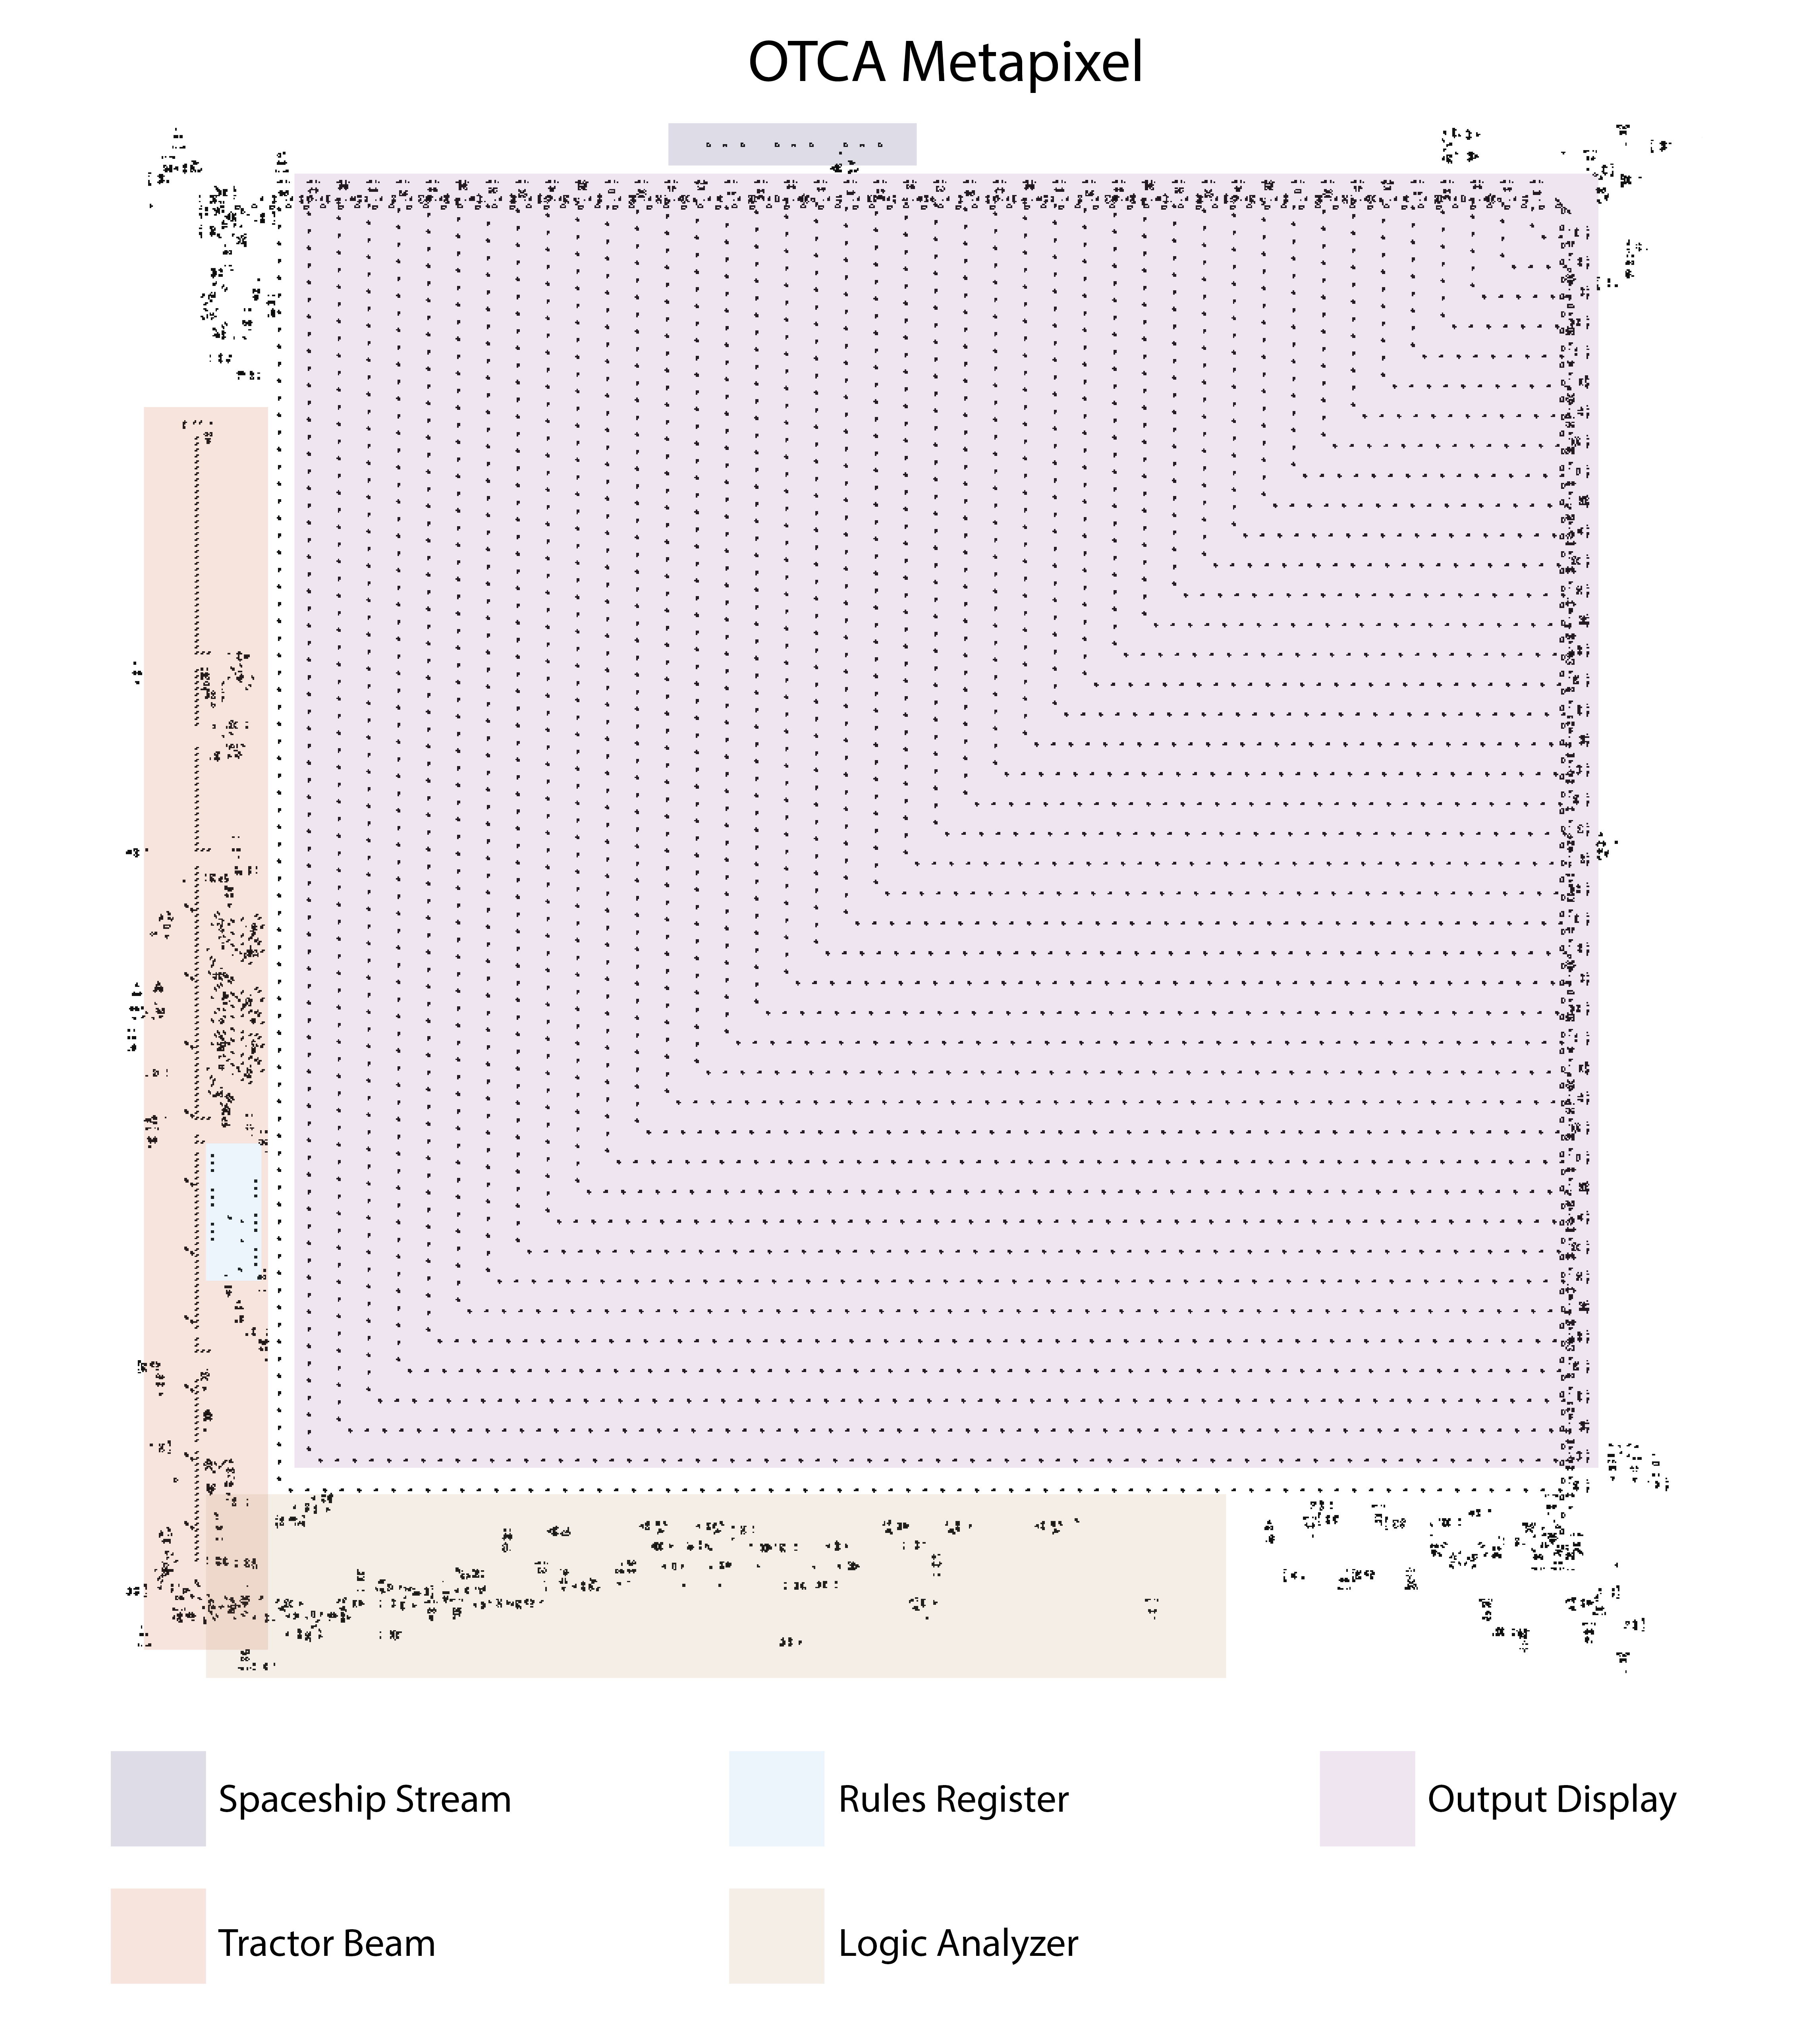
\includegraphics[width=\textwidth]{OTCADiagram.png}
  \caption{System level diagram of OTCA Metapixel with the most important modules highlighted.}
  \label{fig:OTCADiagram}
\end{figure}

\begin{sidewaysfigure}
  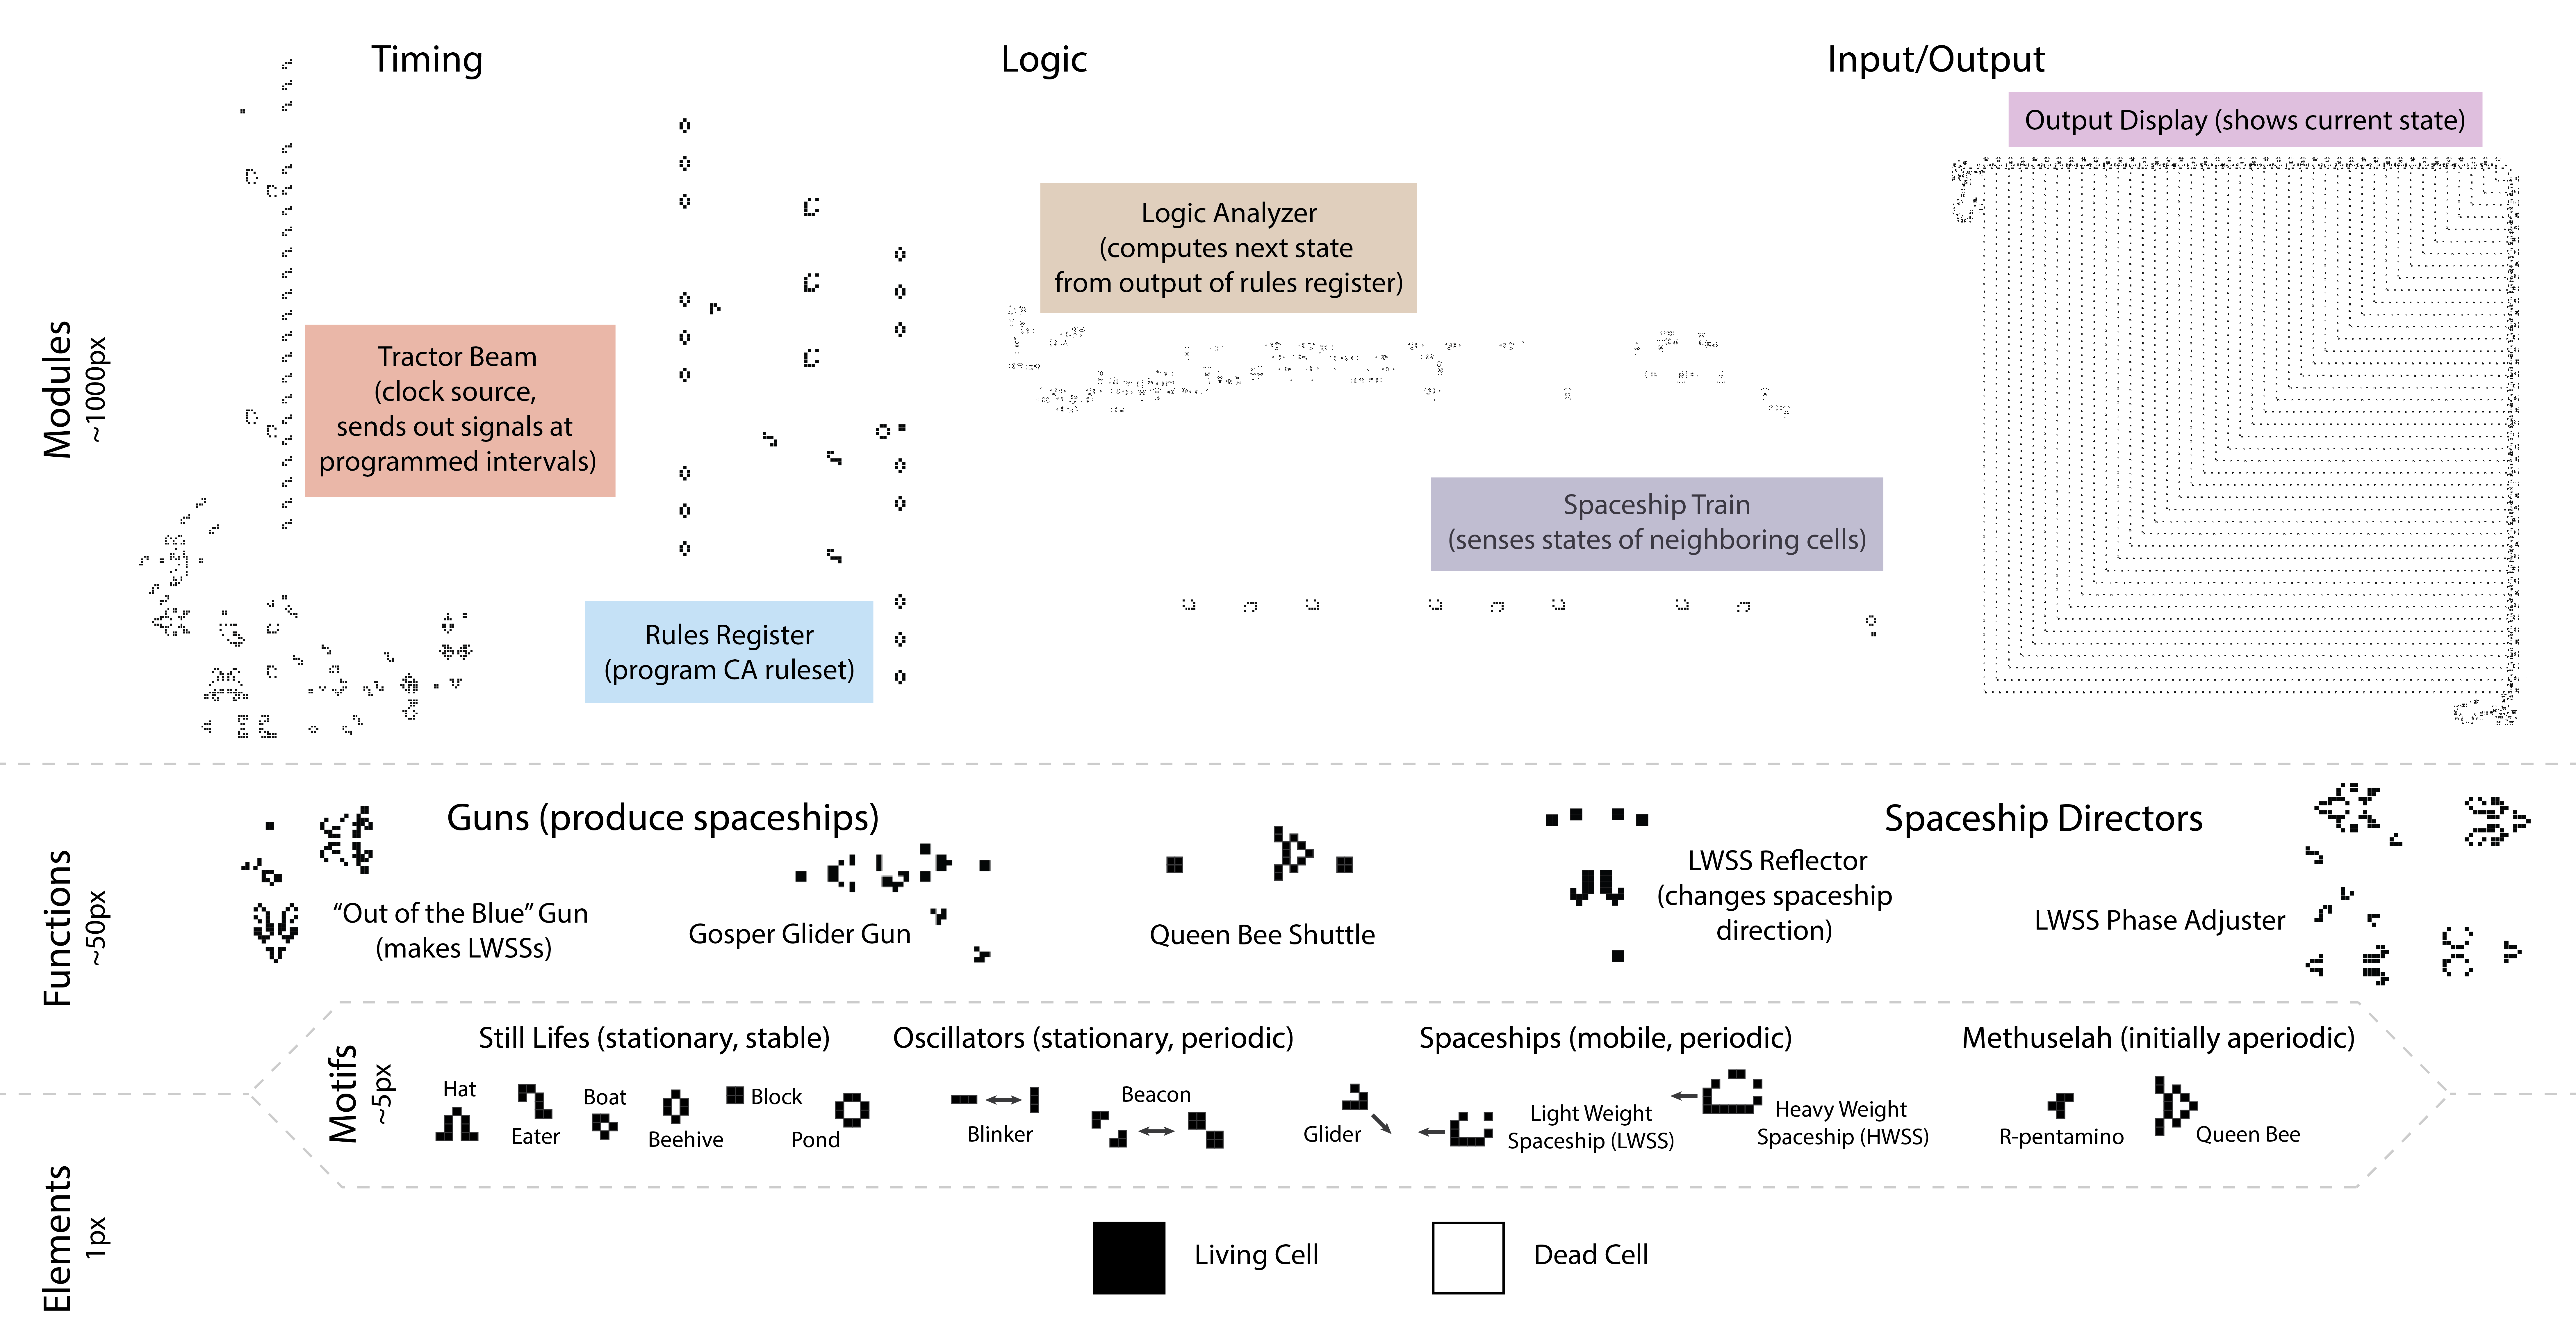
\includegraphics[width=\textwidth,height=\textheight,keepaspectratio]{OTCAMetaHierarchy.png}
  \caption{Hierarchical breakdown of OTCA Metapixel.}
  \label{fig:OTCAMetaHierarchy}
\end{sidewaysfigure}

\section{Electronic Versus Mechanical Hierarchies}

scaling mismatch between the functional density of electronic and mechanical systems, offset in hierarchical setup.

\section{Hierarchy in Simulation}

increasing simulation abstraction as hierarchical level increases\\

In the next chapters, I'll describe the methods used to simulate parts and functions, and describe how abstractions of the parts-level simulation are adapted to the functions-level.



}
